\begin{name}{ĐỀ THAM KHẢO-HXN}{ĐÈ ÔN TẬP TN THPT}\end{name}
\Opensolutionfile{ans}[ans/ans\currfilebase]
%================================PHẦN I
\caulc
\begin{ex}%%[TeX hóa đề tham khảo Hoàng Xuân Nhàn]%[BCTuan, dự án 12-Tex-Hoa-2025]%[2D1N1-2]%Câu 1
\immini
{
		Cho hàm số $y=f(x)$ có đồ thị là đường cong trong hình bên. Hàm số đã cho đồng biến trên khoảng nào dưới đây?
	\choice
	{\True $(0;1)$}
	{$(-\infty;0)$}
	{$(1;+\infty)$}
	{$(-1;0)$}
}
{
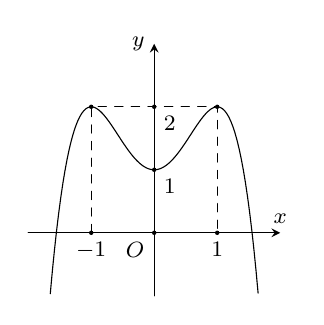
\begin{tikzpicture}[line cap=round,line join=round,font=\footnotesize,>=stealth,scale=0.8]
	\draw[->] (-2,0)--(2,0) node[above] {$x$};
	\draw[->] (0,-1)--(0,3) node[left] {$y$};
	\fill (0,0) circle (1pt) node [below left] {$O$}
	(-1,0) circle (1pt) node [below] {$-1$}
	(1,0) circle (1pt) node [below] {$1$}
	(0,1) circle (1pt) node [below right] {$1$}
	(0,2) circle (1pt) node [below right] {$2$}
	(1,2) circle (1pt) (-1,2) circle (1pt) (0,1) circle (1pt);
	\draw [samples=100, domain=-1.65:1.65] plot (\x, {-(\x)^4+2*(\x)^2+1});
	\draw[dashed] (-1,0)|-(0,2)-|(1,0);
\end{tikzpicture}
}
	\loigiai{
		Hàm số có đồ thị trong hình vẽ trên đồng biến trên các khoảng $(-\infty;-1)$ và $(0;1)$.
	}
\end{ex}

\begin{ex}%%[TeX hóa đề tham khảo Hoàng Xuân Nhàn]%[BCTuan, dự án 12-Tex-Hoa-2025]%[1D5N2-2]%Câu 2
	Thống kê điểm kiểm tra giữa kỳ 1 môn Toán của $30$ học sinh lớp $12$C1 của một trường THPT được ghi lại ở bảng sau
\begin{center}
	\begin{tabular}{|c|c|c|c|c|}
		\hline
		Điểm & $[2;4)$ & $[4;6)$ & $[6;8)$ & $[8;10)$\\
		\hline
		Số học sinh & $4$ & $8$ & $11$ & $7$\\
		\hline
\end{tabular}
\end{center}
	Trung vị của mẫu số liệu gốc thuộc khoảng nào trong các khoảng dưới đây?
	\choice
	{$[2;4)$}
	{$[4;6)$}
	{\True $[6;8)$}
	{$[8;10)$}
	\loigiai{
		Ta có mẫu số liệu trên có tất cả là $30$ học sinh nên trung vị bằng $\dfrac{x_{15}+x_{16}}{2}\in [6;8)$.
	}
\end{ex}

\begin{ex}%%[TeX hóa đề tham khảo Hoàng Xuân Nhàn]%[BCTuan, dự án 12-Tex-Hoa-2025]%[2H5N1-2]%Câu 3
	Trong không gian $Oxyz$, một véc-tơ pháp tuyến của mặt phẳng $\dfrac{x}{-2}+\dfrac{y}{-1}+\dfrac{z}{3}=1$ là
	\choice
	{\True $\overrightarrow{n}=(3;6;-2)$}
	{$\overrightarrow{n}=(2;-1;3)$}
	{$\overrightarrow{n}=(-3;-6;-2)$}
	{$\overrightarrow{n}=(-2;-1;3)$}
	\loigiai{
		Ta có $\dfrac{x}{-2}+\dfrac{y}{-1}+\dfrac{z}{3}=1\Leftrightarrow 3x+6y-2z+6=0$.\\
		Từ đó suy ra một véc-tơ pháp tuyến của mặt phẳng là $\overrightarrow{n}=(3;6;-2)$.
	}
\end{ex}

\begin{ex}%%[TeX hóa đề tham khảo Hoàng Xuân Nhàn]%[BCTuan, dự án 12-Tex-Hoa-2025]%[1D2H2-6]%Câu 4
	Cho cấp số cộng $(u_n)$ với số hạng đầu $u_1=-6$ và công sai $d=4$. Tính tổng $S$ của $14$ số hạng đầu tiên của cấp số cộng đó.
	\choice
	{$S=46$}
	{$S=308$}
	{$S=644$}
	{\True $S=280$}
	\loigiai{
		Tổng $n$ số hạng đầu tiên của một cấp số cộng là $S_n=\dfrac{\left[2u_1+(n-1)d\right]n}{2}$.\\
		Vậy $S_{14}=\dfrac{\left[2\cdot (-6)+(14-1)\cdot 4\right]14}{2}=280$.
	}
\end{ex}

\begin{ex}%%[TeX hóa đề tham khảo Hoàng Xuân Nhàn]%[BCTuan, dự án 12-Tex-Hoa-2025]%[2H2H1-3]%Câu 5
	Cho tứ diện đều $ABCD$ có cạnh bằng $a$. Tích vô hướng $\overrightarrow{AB}\cdot\overrightarrow{AC}$ bằng
	\choice
	{$a^2$}
	{$-a^2$}
	{\True $\dfrac{1}{2}{a^2}$}
	{$\dfrac{\sqrt{3}}{2}{a^2}$}
	\loigiai{
		Do $ABCD$ là tứ diện đều cạnh $a$ nên $AB=AC=a$ và $\left(\overrightarrow{AB},\overrightarrow{AC}\right)=60^\circ$.\\
		Ta có $\overrightarrow{AB}\cdot\overrightarrow{AC}=\left|\overrightarrow{AB}\right|\cdot\left|\overrightarrow{AC}\right|\cdot\cos 60^\circ=\dfrac{a^2}{2}$.
	}
\end{ex}

\begin{ex}%%[TeX hóa đề tham khảo Hoàng Xuân Nhàn]%[BCTuan, dự án 12-Tex-Hoa-2025]%[2D1H3-1]%Câu 6
	Giá trị lớn nhất của hàm số $f(x)=x^3-8x^2+16x-9$ trên đoạn $[1;3]$ là 
	\choice
	{$\max\limits_{[1;3]}f(x)=0$}
	{\True $\max\limits_{[1;3]}f(x)=\dfrac{13}{27}$}
	{$\max\limits_{[1;3]}f(x)=-6$}
	{$\max\limits_{[1;3]}f(x)=5$}
	\loigiai{
		Hàm số đã cho liên tục trên đoạn $[1;3]$.\\
		Ta có $f'(x)=3x^2-16x+16=0$; $f'(x)=0\Leftrightarrow\hoac{&
			x=\dfrac{4}{3}\in (1;3)\\
			&
			x=4\notin (1;3).}$\\
		Ta có $f(1)=0$; $f\left(\dfrac{4}{3}\right)=\dfrac{13}{27}$; $f(3)=-6$.\\ 
		Do đó $\max\limits_{[1;3]}f(x)=\dfrac{13}{27}$.
	}
\end{ex}

\begin{ex}%%[TeX hóa đề tham khảo Hoàng Xuân Nhàn]%[BCTuan, dự án 12-Tex-Hoa-2025]%[2D6H1-2]%Câu 7
	Trong một phép thử với $A$, $B$ là hai biến cố bất kì, biết rằng $\mathrm{P}(A)=0{,}5$; $\mathrm{P}(AB)=0{,}3$. Khi đó $\mathrm{P}\left(B\mid A\right)$ bằng
	\choice
	{\True $0{,}6$}
	{$0{,}15$}
	{$0{,}7$}
	{$0{,}35$}
	\loigiai{
		Ta có $\mathrm{P}\left(B\mid A\right)=\dfrac{\mathrm{P}(AB)}{\mathrm{P}(A)}=\dfrac{0{,}3}{0{,}5}=0{,}6$.
	}
\end{ex}

\begin{ex}%%[TeX hóa đề tham khảo Hoàng Xuân Nhàn]%[BCTuan, dự án 12-Tex-Hoa-2025]%[2D4N2-1]%Câu 8
	Cho biết $\displaystyle\int\limits_1^3f(x)\mathrm{\,d}x=3$, giá trị của $\displaystyle\int\limits_1^3\dfrac{1}{3}f(x)\mathrm{\,d}x$ bằng
	\choice
	{$2$}
	{\True $1$}
	{$\dfrac{1}{3}$}
	{$3$}
	\loigiai{
		Ta có $\displaystyle\int\limits_1^3\dfrac{1}{3}f(x)\mathrm{\,d}x=\dfrac{1}{3}\displaystyle\int\limits_1^3f(x)\mathrm{\,d}x=\dfrac{1}{3}\cdot 3=1$.
	}
\end{ex}

\begin{ex}%%[TeX hóa đề tham khảo Hoàng Xuân Nhàn]%[BCTuan, dự án 12-Tex-Hoa-2025]%[1D6N4-2]%Câu 9
	Tập nghiệm của bất phương trình $2^x\le 4$ là
	\choice
	{\True $(-\infty;2]$}
	{$[0;2]$}
	{$(-\infty;2)$}
	{$(0;2)$}
	\loigiai{
		Ta có $2^x\le 4\Leftrightarrow x\le \log_24\Leftrightarrow x\le 2$.\\
		Tập nghiệm bất phương trình là $S=(-\infty;2]$.
	}
\end{ex}

\begin{ex}%%[TeX hóa đề tham khảo Hoàng Xuân Nhàn]%[BCTuan, dự án 12-Tex-Hoa-2025]%[2D4H1-2]%Câu 10
	Phát biểu nào sau đây là đúng?
	\choice
	{$\displaystyle\int\dfrac{1}{x} \mathrm{\,d}x=|x|+C$}
	{\True $\displaystyle\int\dfrac{1}{x} \mathrm{\,d}x=\ln|x|+C$}
	{$\displaystyle\int\ln x\mathrm{\,d}x=x+C$}
	{$\displaystyle\int\ln|x|\mathrm{\,d}x=\ln x+C$}
	\loigiai{
		Ta có $\displaystyle\int\dfrac{1}{x} \mathrm{\,d}x=\ln|x|+C$.
	}
\end{ex}

\begin{ex}%%[TeX hóa đề tham khảo Hoàng Xuân Nhàn]%[BCTuan, dự án 12-Tex-Hoa-2025]%[2D3H2-2]%Câu 11
	Bạn An rất thích nhảy hiện đại. Thời gian tập nhảy mỗi ngày của bạn An được thống kê lại ở bảng sau:
	\begin{center}
	\begin{tabular}{|l|c|c|c|c|c|}
		\hline {\bf Thời gian (phút)} & {$[20;25)$}&{$[25;30)$}&{$[30;35)$}&{$[35;40)$}&{$[40;45)$}\\
		\hline {\bf Số ngày} & $6$ & $6$ & $4$ & $1$ & $1$ \\
		\hline
	\end{tabular}
	\end{center}
	Độ lệch chuẩn của mẫu số liệu ghép nhóm có giá trị gần nhất với giá trị nào dưới đây?
	\choice
	{$31{,}25$}
	{$31{,}26$}
	{$5{,}4$}
	{\True $5{,}6$}
	\loigiai{
		Giá trị trung bình của mẫu số liệu ghép nhóm là $\overline{x}=\dfrac{22{,}5\cdot 6+27{,}5\cdot 6+\ldots +42{,}5\cdot 1}{18}=\dfrac{85}{3}$.\\
		Độ lệch chuẩn mẫu số liệu ghép nhóm là $$s=\sqrt{s^2}=\sqrt{\dfrac{(22{,}5-\overline{x})^2\cdot 6+(27{,}5-\overline{x})^2\cdot 6+\ldots +(42{,}5-\overline{x})^2\cdot 1}{18}}=\sqrt{\dfrac{125}{4}}\approx 5{,}6.$$
	}
\end{ex}

\begin{ex}%%[TeX hóa đề tham khảo Hoàng Xuân Nhàn]%[BCTuan, dự án 12-Tex-Hoa-2025]%[2H5H2-5]%Câu 12
	Trong không gian $Oxyz$, cho đường thẳng $\Delta \colon \dfrac{x-2}{-3}=\dfrac{y}{1}=\dfrac{z+1}{2}$. Gọi $M$ là giao điểm của $\Delta $ với mặt phẳng $(P)\colon x+2y-3z+2=0$. Tọa độ điểm $M$ là
	\choice
	{$M(2;0;-1)$}
	{$M(5;-1;-3)$}
	{$M(1;0;1)$}
	{\True $M(-1;1;1)$}
	\loigiai{
		Tọa độ điểm $M=\Delta\cap(P)$ là nghiệm của hệ phương trình $$\heva{&
			\dfrac{x-2}{-3}=\dfrac{y}{1}=\dfrac{z+1}{2}\\&
			x+2y-3z+2=0}\Leftrightarrow\heva{&
			\dfrac{x-2}{-3}=\dfrac{y}{1}\\&
			\dfrac{y}{1}=\dfrac{z+1}{2}\\&
			x+2y-3z+2=0} \Leftrightarrow\heva{&
			x+3y=2\\&
			2y-z=1\\&
			x+2y-3z=-2} \Leftrightarrow\heva{&
			x=-1\\&
			y=1\\&
			z=1.}$$ 
	Vậy $M(-1;1;1)$.}
		\end{ex}

%================================PHẦN II
\cauds
\begin{ex}%%[TeX hóa đề tham khảo Hoàng Xuân Nhàn]%[BCTuan, dự án 12-Tex-Hoa-2025]%[2D6H2-4]
	Năm $2025$, báo Giáo dục đã có cuộc khảo sát tại một trường đại học và thấy rằng có $40\%$ sinh viên quan tâm đến chương trình học bổng A; có $17\%$ trong số những sinh viên quan tâm đến học bổng A cũng đã quan tâm đến học bổng B. Qua khảo sát họ cũng thấy rằng có $20\%$ sinh viên quan tâm đến chương trình học bổng B. Người ta chọn ngẫu nhiên một sinh viên từ trường đại học này để thăm dò ý kiến.
	\choiceTF
	{Xác suất để sinh viên được được chọn quan tâm cả hai chương trình học bổng bằng $0{,}062$}
	{Xác suất để sinh viên quan tâm học bổng A nếu biết rằng họ đã quan tâm học bổng B bằng $0{,}4$}
	{Xác suất để sinh viên không quan tâm đến cả chương trình A lẫn học chương trình B bằng $0{,}41$}
	{\True Sinh viên được chọn cho rằng mình có quan tâm đến học bổng B; hai hôm sau một nhà báo khác quay lại trường và tiếp tục chọn ngẫu nhiên một sinh viên để thăm dò ý kiến thì gặp được một sinh viên quan tâm đến học bổng B, xác suất để người này không quan tâm đến học bổng A bằng $0{,}66$}
	\loigiai{
		Gọi $A$ là biến cố: \lq\lq Sinh viên quan tâm đến học bổng A\rq\rq\ và $B$ là biến cố: \lq\lq Sinh viên quan tâm đến học bổng B\rq\rq.\\
		Theo giả thiết ta có $\mathrm{P}(A)=0{,}4$; $\mathrm{P}(B\mid A)=0{,}17$; $\mathrm{P}(B)=0{,}2$.\\
		Từ đây ta có sơ đồ hình cây như sau:
		\begin{center}
			\begin{tikzpicture}[scale=.2,>=stealth]
				\tikzstyle{block}=[rectangle, draw, fill=blue!10{,} rounded corners, text centered, text width=10em, minimum height=2em]
				\node (c1) {};
				\node (c2)[above right=1.5cm of c1] {$A$};
				\node at (0.5,5){$0{,}4$};
				\node at (0.5,-5){$0{,}6$};
				\node (c3) [below right= 1.5cm of c1]{$\overline{A}$};
				\node at (12,11.5){$0{,}17$};
				\node (c4) at (21.5, 12){$B$};
				\node (c5) at (21.5, 2){$\overline{B}$};
				\node at (12,3){$0{,}83$};
				\node (c6) at (21.5, -4){$B$};
				\node at (12,-4){?};
				\node (c7) at (21.5, -14){$\overline{B}$};
				\node at (12,-13){?};
				\draw[->] (c1.east) -- (c2.west);
				\draw[->] (c1.east) -- (c3.west);
				\draw[->] (c2.east) -- (c4.west);
				\draw[->] (c2.east) -- (c5.west);
				\draw[->] (c3.east) -- (c6.west);
				\draw[->] (c3.east) -- (c7.west);
			\end{tikzpicture}
		\end{center}
		\begin{itemchoice}
			\itemch 
			Ta có $\mathrm{P}(AB)=\mathrm{P}(A)\cdot \mathrm{P}(B\mid A)=0{,}4\cdot 0{,}17=0{,}068$.
			\itemch 
			Ta có $\mathrm{P}(A\mid B)=\dfrac{\mathrm{P}(AB)}{\mathrm{P}(B)}=\dfrac{0{,}068}{0{,}2}=0{,}34$.
			\itemch 
			Ta có $\mathrm{P}(A\cup B)=\mathrm{P}(A)+\mathrm{P}(B)-\mathrm{P}(AB)=0{,}4+0{,}2-0{,}068=0{,}532$.\\
			Do đó $\mathrm{P}(\overline{A}\overline{B})=1-\mathrm{P}(A\cup B)=1-0{,}532=0{,}468$.
			\itemch
			Ta có $\mathrm{P}(\overline{A}\mid B)=\dfrac{\mathrm{P}(\overline{A}B)}{\mathrm{P}(B)}=\dfrac{\mathrm{P}(B)-\mathrm{P}(AB)}{\mathrm{P}(B)}=\dfrac{0{,}2-0{,}068}{0{,}2}=0{,}66$.\\
			Vì hai cuộc khảo sát là độc lập nên lần chọn đầu không ảnh hưởng đến lần chọn sau, xác suất cần tính là $\mathrm{P}(\overline{A}\mid B)=0{,}66$.
		\end{itemchoice}
	}
\end{ex}

\begin{ex}%%[TeX hóa đề tham khảo Hoàng Xuân Nhàn]%[BCTuan, dự án 12-Tex-Hoa-2025]%[2D4H3-3]
	Cho hàm số $y=\mathrm{e}^x$ có đồ thị $(C)$. Hình phẳng $(H)$ giới hạn bởi các đồ thị $(C)$, tiếp tuyến của $(C)$ tại điểm $M(1;\mathrm{e})$ và đường thẳng $y=-\dfrac{1}{\mathrm{e}}x$ được tô đậm như hình vẽ.
	\begin{center}
		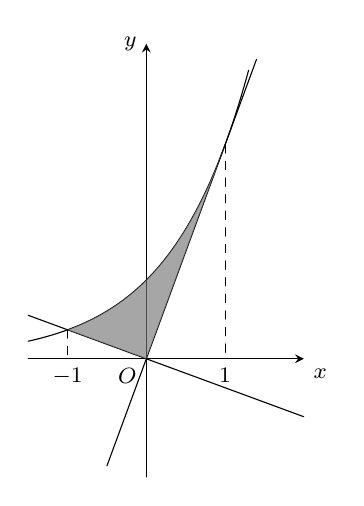
\begin{tikzpicture}[x=1cm,y=1cm,scale=1,line cap=round,line join=round,>=stealth,font=\footnotesize]
			\path (-1,0)coordinate[label=below:$-1$](-1) (1,0)coordinate[label=below:$1$](1);
			\draw[->] (-1.5,0)--(2,0)node[below right]{$x$};
			\draw[->] (0,-1.5)--(0,4)node[left]{$y$};
			\fill (0,0)node[below left]{ $O$};
			\draw[black,samples=150,smooth,domain=-1.5:2] plot(\x,{(-0.368)*(\x)});
			\draw[black,samples=150,smooth,domain=-1.5:1.3] plot(\x,{(2.718)^(\x)});
			\draw[black,samples=150,smooth,domain=-0.5:1.4] plot(\x,{(2.718)*(\x)});
			\draw[dashed] (-1,0.368)--(-1,0)  (1,2.718)--(1,0);
			\fill[gray, opacity=0.7] plot[domain=-1:0] (\x, {(-0.368)*(\x)}) -- plot[domain=0:-1] (\x, {(2.718)^(\x)}) -- cycle;
			\fill[gray, opacity=0.7] plot[domain=0:1] (\x, {(2.718)*(\x)}) -- plot[domain=1:0] (\x, {(2.718)^(\x)}) -- cycle;
		\end{tikzpicture}
	\end{center}
	\choiceTF
	{Phương trình tiếp tuyến của $(C)$ tại điểm $M(1;\mathrm{e})$ là $y=\mathrm{e}x+\mathrm{e}$}
	{\True Đường thẳng $y=-\dfrac{1}{\mathrm{e}}x$ cắt đồ thị tại điểm $\left(-1;\dfrac{1}{\mathrm{e}}\right)$}
	{\True Diện tích hình phẳng $(H)$ bằng $0{,}81$ (\textit{làm tròn đến hàng phần trăm})}
	{Khi quay hình $(H)$ quanh trục hoành thì được khối tròn xoay có thể tích bằng $3{,}03$ (\textit{làm tròn đến hàng phần trăm})}
	\loigiai{
		\begin{itemchoice}
			\itemch
			Phương trình tiếp tuyến của $(C)$ tại điểm $M(1;\mathrm{e})$ là $y=y'(1)(x-1)+\mathrm{e}$ hay $y=\mathrm{e}x$.
			\itemch 
			Tọa độ giao điểm của $(C)$ và đường thẳng $y=-\dfrac{1}{\mathrm{e}}x$ thỏa mãn $\heva{&\mathrm{e}^x=-\dfrac{1}{\mathrm{e}}x\\&y=\mathrm{e}^x} \Leftrightarrow \heva{&x=-1\\&y=\mathrm{e}^{-1}=\dfrac{1}{\mathrm{e}}.}$\\
			{\bf Giải thích:} Phương trình $\mathrm{e}^x=-\dfrac{1}{\mathrm{e}}x$ có hai vế là các hàm số $y=\mathrm{e}^x$ đồng biến trên $\mathbb{R}$; $y=-\dfrac{1}{\mathrm{e}}x$ nghịch biến trên $\mathbb{R}$ nên có tối đa một nghiệm, nghiệm đó là $x=-1$.
			\itemch 
			Dễ thấy đường thẳng $y=\mathrm{e}x$ cắt đường thẳng $y=-\dfrac{1}{\mathrm{e}}x$ tại điểm có hoành độ $x=0$ và cắt đồ thị $(C)$ tại điểm có hoành độ $x=1$.\\
			Do đó diện tích hình phẳng $(H)$ là
			$$S=\displaystyle\int\limits_{-1}^0\left(\mathrm{e}^x+\dfrac{1}{\mathrm{e}}x\right)\mathrm{d}x+\displaystyle\int\limits_0^1\left(\mathrm{e}^x-\mathrm{e}x\right)\mathrm{d}x \approx 0{,}81.$$
			\itemch 
			Thể tích khối tròn xoay là
			$$V=\pi \displaystyle\int\limits_{-1}^1\left(\mathrm{e}^x \right)^2\mathrm{d}x-\pi \displaystyle\int\limits_{-1}^0\left(-\dfrac{1}{\mathrm{e}}x\right)^2\mathrm{d}x-\pi \displaystyle\int\limits_0^1(\mathrm{e}x)^2\mathrm{d}x \approx 3{,}51.$$
		\end{itemchoice}
	}
\end{ex}

\begin{ex}%%[TeX hóa đề tham khảo Hoàng Xuân Nhàn]%[BCTuan, dự án 12-Tex-Hoa-2025]%[2D1V3-6]
	Hai thành phố cách nhau một con sông. Lấy $A$ và $B$ lần lượt là hai điểm mốc của hai thành phố trong việc đo đạc, đơn vị là km. Người ta xây dựng một cây cầu $EF$ bắc qua sông biết rằng vị trí $A$ cách con sông một khoảng $AH=5$ km và vị trí B cách con sông một khoảng là $BK= 7$ km (xem hình vẽ), biết $HE+KF=24$ km và độ dài $EF$ không đổi. Đặt $HE=x$ (km), với $x\in (0; 24)$.
	\begin{center}
		\begin{tikzpicture}[line cap=round,line join=round,scale=0.9,font=\footnotesize,>=stealth]
			\coordinate (a) at (0,0);
			\coordinate (b) at (2,0);
			\coordinate (c) at (0,4);
			\coordinate (d) at (2,4);
			\path[draw,fill=cyan!90!blue,fill opacity=0.35] (a) rectangle (d);
			\coordinate (E) at (0,1);
			\coordinate (H) at (0,3);
			\coordinate (K) at (2,0.5);
			\coordinate (F) at (2,1);
			\coordinate (A) at (-2,3);
			\coordinate (B) at (4,0.5);
			\draw (F)--(B)--node[below]{$7$}(K);
			\draw (E)--(A)--node[above]{$5$}(H)--node[left]{$x$}(E);
			\draw[line width=4pt] (E)--(F);
			\foreach \x/\y in {A/180,E/200,H/120, K/-45, F/45, B/0}{\fill (\x) circle(1pt) ($(\x)+(\y:0.3cm)$) node{$\x$};}
		\end{tikzpicture}
	\end{center}
	\choiceTF
	{\True $AE=\sqrt{25+x^2}$ (km), $BF=\sqrt{49+(24-x)^2}$ (km)}
	{Tổng quãng đường đi từ $A$ đến $B$ bằng $\sqrt{25+x^2}+\sqrt{49+x^2}+EF$ (km)}
	{\True Nếu đặt $f(x)=AE+BF$ (km) thì $f'(x)=\dfrac{x}{\sqrt{x^2+25}}+\dfrac{x-24}{\sqrt{x^2-48x+625}}$, $\forall x\in (0; 24)$}
	{Người ta muốn đi từ $A$ đến $B$ theo quãng đường ngắn nhất thì họ phải xây cầu sao cho khoảng cách hai điểm $E$, $H$ bằng $9$ km}
	\loigiai{
		\begin{itemchoice}
			\itemch
			Với $HE=x$ thì $FK=24-x$, ($0< x < 24$).\\
			Ta có $\heva{&AE=\sqrt{25+x^2} \\ &BF=\sqrt{49+(24-x)^2}.}$
			\itemch 
			Tổng quãng đường đi từ $A$ đến $B$ là $$AE+EF+BF=\sqrt{25+x^2}+\sqrt{49+(24-x)^2}+EF\text{ (km)}.$$
			\itemch 
			Xét hàm số $f(x)=\sqrt{x^2+25}+\sqrt{x^2-48x+625}$.\\
			Ta có
			$$f'(x)=\dfrac{x}{\sqrt{x^2+25}}+\dfrac{x-24}{\sqrt{x^2-48x+625}}, \forall x\in (0; 24).$$
			\itemch 
			Ta cần tổng quãng đường $AE+EF+FB$ ngắn nhất, mà $EF$ không đổi nên $AE+FB$ bé nhất.\\
			Ta có $f'(x)=\dfrac{x}{\sqrt{x^2+25}}+\dfrac{x-24}{\sqrt{x^2-48x+625}}, \forall x\in (0; 24)$.\\
			Và $f'(x)=0\Leftrightarrow x=10$.\\
			Bảng biến thiên:
			\begin{center}
				
\begin{tikzpicture}
					\tkzTabInit[nocadre=false, lgt=1.2, espcl=2, deltacl=0.6]
					{$x$/0.8,$f'(x)$/0.8,$f(x)$/2.3}
					{$0$,$10$,$24$};
					\tkzTabLine{,-,$0$,+,};
					\tkzTabVar{+/,-/$12\sqrt{5}$,+/};
				\end{tikzpicture}
			\end{center}
			Ta có $\min\limits_{(0 ; 24)} f(x)=12 \sqrt{5}$, khi đó $x=10$ km và $B F=7 \sqrt{5}\approx 15{,}65$ km.
		\end{itemchoice}
	}
\end{ex}

\begin{ex}%%[TeX hóa đề tham khảo Hoàng Xuân Nhàn]%[BCTuan, dự án 12-Tex-Hoa-2025]%[2H5V3-4]
	Trong Dragon Ball, quả cầu Genki là chiêu thức lợi hại mà SonGoku thường sử dụng khi gặp những đối thủ lớn. Được biết trong trận đánh với Frieza đại đế, cuộc chiến có liên quan đến vận mệnh vũ trụ, Goku đã dùng quả cầu này để tung đòn tuyệt sát với Frieza.
	Chọn hệ trục tọa độ $Oxyz$ thích hợp, đơn vị trên mỗi trục là mét, mặt phẳng $Oxy$ là mặt đất và tia $Oz$ hướng lên trời, SonGoku đứng ở vị trí $A(5;0;40)$, Frieza đại đế đứng ở vị trí $B(85;60;40)$. Trước khi Goku tạo ra quả cầu Genki thì Frieza đã tấn công phủ đầu, hắn lao về phía Goku với vận tốc $50$ m/s.
	\choiceTF
	{\True Frieza sẽ mất $2$ giây để đến được vị trí Goku đang đứng}
	{Véc-tơ vận tốc của Frieza là $\overrightarrow{v}=(400;300;0)$, đơn vị: m/s}
	{\True Sau khi tránh được đòn hiểm từ Frieza, Goku đứng ở vị trí $C(8;-1; 46)$ đã tạo ra quả cầu Genki được mô hình hóa với phương trình $(x-8)^2+(y+1)^2+(z-58)^2=100$. Khoảng cách bé nhất từ vị trí $D(-182; 159; 45)$ mà Frieza đang đứng đến quả cầu bằng $238{,}7$ m \textit{(kết quả làm tròn đến hàng phần chục)}}
	{\True Quả cầu được Goku ném về phía Frieza với vận tốc lên đến $64$ m/s. Cứ sau mỗi giây thì bán kính nó tăng lên $1$ mét. Nếu Frieza không di chuyển thì sau $3{,}67$ giây thì quả cầu Genki đến được vị trí của Frieza \textit{(làm tròn đến hàng phần trăm của giây)}}
	\loigiai{
		\begin{itemchoice}
			\itemch 
			Ta có $\overrightarrow{BA}=(-80;-60; 0)$ và $AB=\sqrt{(-80)^2+(-60)^2}=100$ (m).\\
			Thời gian để Frieza bay từ $B$ đến $ A$ để tấn công Goku là $\dfrac{100}{50}=2$.
			\itemch 
			Véc-tơ vận tốc của Frieza có dạng $\overrightarrow{v}=k\overrightarrow{BA}=(-80k;-60k; 0)$, với tham số $k > 0$.\\
			Ta có $\left|\overrightarrow{v}\right|=50\Leftrightarrow \sqrt{(-80k)^2+(-60k)^2}=50\Leftrightarrow 100k=50\Leftrightarrow k=\dfrac{1}{2}>0$.\\
			Do đó Frieza bay đến chỗ Goku với véc-tơ vận tốc $\overrightarrow{v}=(-40;-30; 0)$.
			\itemch Hình vẽ như sau:
			\begin{center}
				\begin{tikzpicture}[line cap=round,line join=round,scale=0.9,font=\footnotesize,>=stealth]
					\coordinate (I) at (0,0);
					\draw (I) circle (2cm);
					\coordinate (M) at (2,0);
					\coordinate (D) at (5,0);
					\draw (I)--node[above]{$R$}(M)--(D);
					\foreach \x/\y in {I/180, M/45, D/0}{\fill (\x) circle(1pt) ($(\x)+(\y:0.3cm)$) node{$\x$};}
				\end{tikzpicture}
			\end{center}
			Quả cầu Genki có tâm $I(8;-1;58)$, bán kính $R=10$ m.\\
			$ID=\sqrt{(-182-8)^2+(159+1)^2+(45-58)^2}=\sqrt{61\,869} \approx 248{,}7$.\\
			Khoảng cách ngắn nhất cần tính là $MD=ID-R=\sqrt{61\,869}-10\approx 238{,}7$ (m).
			\itemch 
			Sau $t$ giây, điểm $M$ (thuộc mặt cầu gần Frieza nhất) di chuyển đoạn đường $64t+t=65t$ (m).\\
			Khi $M$ chạm vào Frieza (nếu hắn đứng yên) thì $ID-R=65t\Rightarrow t=\dfrac{ID-R}{65} \approx 3{,}67$ (giây).
		\end{itemchoice}
	}
\end{ex}

%================================PHẦN III
\caukq
\begin{ex}%%[TeX hóa đề tham khảo Hoàng Xuân Nhàn]%[BCTuan, dự án 12-Tex-Hoa-2025]%[1H8V7-9]
	\immini[thm]{Một cái ly nước hình hình trụ có chiều cao $9$ cm. Lượng nước trong ly chiếm $\dfrac{2}{3}$ thể tích ly nước. Bạn Hoa đặt một viên kim cương hình lập phương vào miệng ly nước thì thấy một đỉnh của viên kim cương chạm vào mặt nước, đồng thời mô hình ly nước và kim cương cùng lấy trục ly nước làm trục đối xứng. Nếu ban đầu Hoa đổ nước đầy ly thì sau khi đặt khối lập phương như trên, lượng nước tràn ra là bao nhiêu cm khối ({\it làm tròn đến hàng phần chục và bỏ qua độ dày của ly})?	
	}
	{
\begin{tikzpicture}[>=stealth, line join=round, line cap=round, font=\footnotesize, scale=0.45,blue]
	%----------- đn số
	\def\x{2.2} % Bán kính trụ lớn
	\pgfmathsetmacro{\y}{0.3*\x} % Bán kính trục bé
	\def\h{4.2} % Chiều cao
	%---------- tô ly
	\def\tiso{0.33}
	\draw[teal,fill=cyan!7,line width=1.5pt] (\x,0) coordinate (A) --(\x,-\h) coordinate (A1) 	arc(0:-180:\x cm and \y cm) coordinate (B1) --(-\x,0) coordinate (B) arc(180:0:\x cm and \y cm);
	\draw[teal,line width=2pt] (0,0) ellipse (\x cm and \y cm);
	% nước
	\draw[teal,fill=cyan!25] (\x,-\tiso*\h) coordinate (An) --(\x,-\h) arc(0:-180:\x cm and \y cm) --(-\x,-\tiso*\h) coordinate (Bn) arc(180:0:\x cm and \y cm);
	\draw[teal,fill=cyan!40] (0,-\tiso*\h) ellipse (\x cm and \y cm);
	% đáy
	\draw[teal,line width=2pt](\x,-\h) arc(0:-180:\x cm and \y cm);
	% lập phương
	\def\cao{2.5}
	\path ($(0,0)+(160:\x cm and \y cm)$) coordinate (BB)
	($(0,0)+(20:\x cm and \y cm)$) coordinate (AA)
	; 	
	\path ($(An)!0.5!(Bn)$) coordinate (tam)
	($(tam)!1.2!(AA)$) coordinate (M)
	($(tam)!1.2!(BB)$) coordinate (N)
	(M)++(0,\cao) coordinate (M1)
	(N)++(0,\cao) coordinate (N1)
	(tam)++(0,\cao) coordinate (tam1)
	($(M1)+(N1)-(tam1)$) coordinate (D)
	;
	\draw[teal,black, top color=gray!10, bottom color=black!70] (tam)--(N)--(N1)--(D)--(M1)--(M)--cycle;
	\draw[teal] (tam)--(tam1);
	\draw[teal,black, left color=gray!10, right color=gray] (N1)--(tam1)--(tam)--(N)--cycle;
	\draw[teal,black, left color=gray, right color=gray!10] (M1)--(tam1)--(tam)--(M)--cycle;
	\draw[teal,line width=2pt] (\x,0) arc(0:-180: \x cm and \y cm);
\end{tikzpicture}
	}
	\par\shortans[0]{23{,}4}
	\loigiai{
		\immini
		{Xét hình chóp tam giác đều $S.ABC$ trong đó $S$ là đỉnh của hình lập phương nằm bên trong ly nước và $A$, $B$, $C$ là các điểm chung của kim cương với miệng ly; $O$ là trọng tâm $\triangle ABC$ và $H$ là trung điểm $BC$.\\
			Đặt $x$ cm là cạnh đáy hình chóp thì $AO=\dfrac{2}{3} AH=\dfrac{2}{3} \cdot \dfrac{x\sqrt{3}}{2}=\dfrac{x\sqrt{3}}{3}$.\\
			Vì hình chóp $S.ABC$ có $SA$, $SB$, $S C$ bằng nhau và đôi một vuông góc tại $S$ nên $SA=SB=SC=\dfrac{x}{\sqrt{2}}$.\\
			Từ đó suy ra $SO=\sqrt{SA^2-OA^2}=\sqrt{\dfrac{x^2}{2}-\dfrac{x^2}{3}}=\dfrac{x \sqrt{6}}{6}$.
		}
		{\begin{tikzpicture}[line join=round,line cap=round,line width=.6pt,font=\footnotesize,scale=1]
				\coordinate[label=left:$A$] (A) at (0,0);
				\coordinate[label=below left:$B$] (B) at (1,-1);
				\coordinate[label=right:$C$] (C) at (4,0);
				\coordinate[label=below right:$H$] (H) at ($(B)!.5!(C)$);
				\coordinate[label=below:$O$] (O) at ($(A)!2/3!(H)$);
				\coordinate[label=above left:$S$] (S) at ($(O)+(90:4)$);
				\draw (A)--(B)--(C)--(S)--cycle (S)--(B);
				\draw[dashed] (H)--(A)--(C) (O)--(S);
				\fill (A)circle(1.2pt) (B)circle(1.2pt) (C)circle(1.2pt) (S)circle(1.2pt) (O)circle(1.2pt) (H)circle(1.2pt);
			\end{tikzpicture}
		}\noindent
		Theo giả thiết thì chiều cao hình chóp $S.ABC$ bằng $\dfrac{1}{3}$ chiều cao ly nước, tức là $SO=\dfrac{1}{3} \cdot 9=3$.\\
		Suy ra $\dfrac{x\sqrt{6}}{6}=3 \Rightarrow x=3 \sqrt{6}$ (cm).\\
		Ta biết rằng thể tích nước tràn ra bằng với thể tích khối chóp $S.ABC$.\\
		Thể tích đó là
		$V=\dfrac{1}{3} SO \cdot S_{\triangle ABC}=\dfrac{1}{3} \cdot 3 \cdot \dfrac{ \left(3\sqrt{6}\right)^2 \sqrt{3}}{4}=\dfrac{27\sqrt{3}}{2} \approx 23{,}4 \ \left(\text{cm}^3\right)$.
	}
\end{ex}

\begin{ex}%%[TeX hóa đề tham khảo Hoàng Xuân Nhàn]%[BCTuan, dự án 12-Tex-Hoa-2025]%[2D1H3-6]
	Một người công nhân có thể sản xuất với tốc độ là $q(t)=100+\mathrm{e}^{-0{,}5t}$ đơn~vị sản phẩm trong một giờ, với $t$ (giờ) là thời gian tính từ khi bắt đầu làm việc. Biết rằng công nhân bắt đầu làm việc từ $8$ giờ sáng, hỏi người đó sản xuất được bao nhiêu đơn vị sản phẩm trong khoảng thời gian từ $9$ giờ sáng đến $11$ giờ trưa ({\it làm tròn đến hàng đơn~vị})?
	\shortans[0]{$201$}
	\loigiai{
		Gọi $Q(t)$ là số đơn~vị sản phẩm mà công nhân sản xuất được sau $t$ giờ tính từ lúc $8$ giờ sáng.\\
		Ta có $Q'(t)=q(t)=100+\mathrm{e}^{-0{,}5t}$.\\
		Số đơn~vị sản phẩm người đó sản xuất được từ $9$ giờ sáng đến $11$ giờ trưa là\\
		$Q(3)-Q(1)=\displaystyle\int\limits_{1}^{3}q(t)  \mathrm{d}t=\displaystyle\int\limits_{1}^{3}\left (100+\mathrm{e}^{-0{,}5t}\right)  \mathrm{d}t\approx201$ (đơn vị sản phẩm).
	}
\end{ex}

\begin{ex}%%[TeX hóa đề tham khảo Hoàng Xuân Nhàn]%[BCTuan, dự án 12-Tex-Hoa-2025]%[2D1V3-6]
	Mảnh đất vườn của nhà anh Điệp có một phần ranh giới cũng là một phần đường cong $(C)\colon y=\dfrac{x+a}{x+b}$, bao quanh nó là sông nước. Với hệ trục tọa độ $Oxy$ thích hợp, đơn~vị trên mỗi trục là $10$ mét thì đường cong $(C)$ đi qua điểm $(2;3)$ và có đường tiệm cận đứng $x=1$. Hàng ngày, anh Điệp phải dùng thuyền máy để vận chuyển trái cây từ khu vườn của mình đến hai tuyến đường $\Delta_1\colon 2x+y-4=0$ và $\Delta_2\colon x+2y-2=0$ cho những người lái buôn từ nơi khác đến. Anh Điệp cần xác định một vị trí $M\left (x_0;y_0\right )$ thuộc khu vườn của mình để tổng các khoảng cách từ vị trí $M$ đó đến hai tuyến đường $\Delta_1$, $\Delta_2$ là bé nhất. Hỏi khoảng cách từ vị trí được chọn làm gốc tọa độ đến điểm $M$ là bao nhiêu mét ({\it làm tròn đến hàng phần chục})?
	\shortans[0]{$34{,}1$}
	\begin{center}
		\begin{tikzpicture}[line cap=round,line join=round,font=\footnotesize,scale=0.9,>=stealth]
			\pgfmathsetmacro\r{sqrt(2)}
			\pgfmathsetmacro\a{(7-\r)/5}
			\pgfmathsetmacro\b{(6+2*\r)/5}
			\pgfmathsetmacro\c{(4+2*\r)/5}
			\pgfmathsetmacro\d{(3-\r)/5}
			\path
			(1+\r,1+\r) coordinate (M)
			(\a,\b) coordinate (A)
			(\c,\d) coordinate (B)
			(0,0) coordinate (O)
			(2,0) coordinate (C)		
			;
			\draw[-stealth] (-3.5,0)--(3.5,0)node[below]{$x$};
			\draw[-stealth] (0,-0.75)--(0,5)node[above]{$y$};
			\draw[smooth] plot[domain=1.5:3.5] (\x, {(\x+1)/(\x-1)});
			\begin{scope}
				\clip  [smooth] plot[domain=1.5:3.5] (\x, {(\x+1)/(\x-1)});
				\fill [pattern=north east lines] (1.5,1.8) rectangle (3.5,5);
			\end{scope}
			\draw[dashed] (A)--(M)--(B);
			\draw
			(-3.5,2.75)--(3.5,-0.75) node[pos=.25,sloped,below]{$\Delta_2\colon x+2y-2=0$}
			(-.5,5)--(2.375,-0.75) node[pos=.25,sloped,below]{$\Delta_1\colon 2x+y-4=0$}
			(1.5,5) node[left] {$(C)$}
			pic[draw,angle radius=2mm]{right angle=M--A--C}
			pic[draw,angle radius=2mm]{right angle=M--B--C}
			;
			\foreach \x/\g in {M/-80,A/90,B/100,O/-135}
			\draw[fill=white] (\x) circle (.05)+(\g:.5) node {$\x$};
		\end{tikzpicture}
	\end{center}
	\loigiai{
Đồ thị hàm số có tiệm cận đứng $x=-b=1\Rightarrow b=-1$.\\
Khi đó đồ thị hàm số $y=\dfrac{x+a}{x-1}$ qua $(2;3)\Rightarrow 3=\dfrac{2+a}{2-1}\Rightarrow a=1$.\\
Vậy hàm số là $(C)\colon y=\dfrac{x+1}{x-1}$.\\
Gọi $M\left(x_0;\dfrac{x_0+1}{x_0-1}\right) \in (C)$, $x_0>1$.\\
Tổng khoảng cách từ $M$ đến hai đường thẳng $\Delta_1$, $\Delta_2$ là
\allowdisplaybreaks
\begin{eqnarray*}
	&&\mathrm{d}=\mathrm{d}\left(M,\Delta_1\right)+\mathrm{d}\left(M, \Delta_2\right)=\dfrac{\left|2x_0+\dfrac{x_0+1}{x_0-1}- 4\right|}{\sqrt{5}}+\dfrac{\left|x_0+2 \cdot \dfrac{x_0+1}{x_0-1}-2\right|}{\sqrt{5}}\\\\
	&\Leftrightarrow & \sqrt{5} \mathrm{d}=\left|\dfrac{2x_0^2-5x_0+5}{x_0-1}\right|+\left|\dfrac{x_0^2-x_0+4}{x_0-1}\right|=\dfrac{2x_0^2-5x_0+5}{x_0-1}+\dfrac{x_0^2-x_0+4}{x_0-1}\\
	&\Leftrightarrow & \heva{&2x_0^2-5x_0+5 > 0 \\&x_0-1 > 0 \\&x_0^2-x_0+4 > 0}, \forall x_0 > 1.
\end{eqnarray*}
Đặt $\sqrt{5}\mathrm{d}= \dfrac{3x_0^2-6x_0+9}{x_0-1}=g(x)$ với $x > 1$.\\
Ta có $g'(x)=\dfrac{3x_0^2-6x_0-3}{\left(x_0-1\right)^2}$.\\
Khi đó $g'(x)=0 \Rightarrow 3x_0^2-6x_0-3=0 \Rightarrow x_0=1+\sqrt{2}>1$.\\
Ta có $\min\limits _{(1; +\infty)} g(x)=g \left(1+\sqrt{2}\right)=6\sqrt{2} \Rightarrow \sqrt{5}\mathrm{d} \geq 6 \sqrt{2} \Rightarrow \mathrm{d} \geq \dfrac{6\sqrt{10}}{5}$.\\
Dấu đẳng thức xảy ra khi $x_0=1+\sqrt{2} \Rightarrow M \left(1+\sqrt{2}; 1+\sqrt{2}\right)$.\\
Khoảng cách $OM$ trên thực tế là $10\sqrt{\left(1+\sqrt{2}\right)^2+\left(1+\sqrt{2}\right)^2}=10 \times\left(1+\sqrt{2}\right) \sqrt{2} \approx 34{,}1$ (m).
}		
\end{ex}

\begin{ex}%%[TeX hóa đề tham khảo Hoàng Xuân Nhàn]%[BCTuan, dự án 12-Tex-Hoa-2025]%[1D7V2-8]
	\immini
	{Một tên trộm đang cố gắng kéo thùng nữ trang qua một bức tường có độ dày $BC=1$ m; biết rằng tường cao $4$m và sợi dây được kéo theo đường gấp khúc $ABCD$ có độ dài không đổi bằng $20$m, đoạn $BF=0{,}5$ m. Trong khi kéo thì tên trộm luôn ghì đầu dây theo một thanh vịn của cầu thang (đầu dây dịch chuyển theo phương $AF$).
	}
	{\begin{tikzpicture}[>=stealth, line join=round, line cap=round, font=\footnotesize, scale=0.9]
			\def\nguoi{
				\tikz[yscale=-1]{%
					\fill[orange] (1.6, 26.7).. controls (1.5, 26.6) and 
					(1.4, 26.5) .. (1.4, 26.3).. controls (1.3, 26.2) and (1.3, 26.0) .. (1.4, 
					25.9) -- (1.3, 25.9).. controls (1.5, 25.8) and (1.9, 25.8) .. (2.1, 26.0).. 
					controls (2.1, 26.0) and (2.0, 26.1) .. (2.0, 26.2).. controls (2.0, 26.3) and
					(2.0, 26.4) .. (1.8, 26.6).. controls (1.8, 26.6) and (1.8, 26.7) .. (1.9, 
					26.7) -- (1.8, 26.8).. controls (1.7, 26.9) and (1.7, 26.8) .. (1.6, 26.7) -- 
					cycle;
					\fill[black] (1.6, 26.7).. controls (1.7, 27.0) and 
					(1.8, 26.8) .. (1.9, 26.7).. controls (1.9, 26.7) and (2.0, 26.7) .. (2.0, 
					26.8).. controls (2.1, 27.1) and (2.0, 27.4) .. (1.8, 27.8).. controls (1.6, 
					28.6) and (1.5, 28.7) .. (1.8, 29.4).. controls (1.8, 29.6) and (1.4, 29.7) ..
					(1.4, 29.5).. controls (1.4, 29.4) and (1.7, 29.6) .. (1.5, 29.1).. controls 
					(1.3, 28.7) and (1.5, 28.4) .. (1.5, 28.1).. controls (1.5, 27.9) and (1.4, 
					27.9) .. (1.3, 28.0).. controls (0.8, 28.5) and (0.8, 28.8) .. (0.6, 29.3).. 
					controls (0.6, 29.5) and (0.3, 29.5) .. (0.2, 29.5).. controls (0.2, 29.4) and
					(0.3, 29.4) .. (0.4, 29.3).. controls (0.6, 29.3) and (0.6, 28.7) .. (0.7, 
					28.4).. controls (0.9, 28.1) and (1.1, 28.0) .. (1.3, 27.7).. controls (1.4, 
					27.5) and (1.5, 27.2) .. (1.4, 27.0).. controls (1.1, 27.1) and (0.7, 27.3) ..
					(0.4, 27.1).. controls (0.1, 27.0) and (0.1, 27.0) .. (0.1, 26.9).. controls 
					(0.0, 26.8) and (0.1, 26.7) .. (0.4, 26.7).. controls (0.3, 27.4) and (1.3, 
					26.8) .. (1.6, 26.7) -- cycle;
					
					\fill (1.3, 25.9).. controls (1.5, 25.3) and 
					(2.0, 25.3) .. (2.1, 26.0).. controls (2.0, 26.1) and (1.9, 26.2) .. (1.8, 
					26.3).. controls (1.7, 26.4) and (1.6, 26.3) .. (1.6, 26.3).. controls (1.5, 
					26.3) and (1.5, 26.3) .. (1.4, 26.3).. controls (1.3, 26.2) and (1.4, 26.1) ..
					(1.4, 26.0).. controls (1.5, 26.1) and (1.5, 26.2) .. (1.9, 26.1).. controls 
					(2.0, 26.1) and (2.0, 26.1) .. (2.0, 26.0).. controls (1.7, 26.0) and (1.4, 
					26.0) .. (1.3, 25.9) -- cycle;
			}}
			%vẽ
			\def\a{8.3}\def\b{0.8} %dưới
			\def\aa{1.4}\def\bb{3} %lớp trên
			\draw[teal,fill=red,draw=red] (0,0) rectangle ++(\a,\b); 
			\fill[pattern={bricks},
			pattern color=white] (0,0) rectangle ++(\a,\b);
			%% hộp
			\path (0.7,\b)coordinate (D);
			\draw[teal,fill=yellow] (D)++(-4mm,0) rectangle ++(8mm,4mm) ++(0,-2mm)coordinate(tam);
			\draw[teal,->,thick,red] (tam)--++(0:0.85cm);
			%%
			\draw[teal,fill=red,draw=red] (2.7,\b) coordinate (E) rectangle ++(\aa,\bb);
			\fill[pattern={bricks},
			pattern color=white] (2.7,\b) coordinate (E) rectangle ++(\aa,\bb);
			\draw[teal,thick] (D)--($(E)+(0,\bb)$) coordinate (C)++(\aa,0) coordinate(B)--(6.5,1.7) coordinate (A);
			\draw[teal,very thick] ($(E)+(\aa,0.7*\bb)$) coordinate (F)--(\a,\b) ++(168:0.9cm)node{\scriptsize $30^\circ$};
			% trộm
			\path (6.4,\b)++(0,-2pt) node[anchor=south west,inner sep=0] (nA) {\resizebox{!}{1.5cm}{\nguoi}};
			% nhẫn
			\foreach \diem/\goc in {D/120,C/90,B/90,A/60,E/135,F/-70} {\fill[black] (\diem) circle (1pt) ++(\goc:0.25) node{$\diem$};}
			\path (B)--(F) node[midway, above=-2pt, sloped]{\tiny $0{,}5$m}%
			(C)--(E) node[midway,left]{$4$ m}
			(C)--(B) node[midway,above]{$1$ m}
			;
			\draw[teal,<-,thick,red] (A)++(-2pt,-5pt)--++(155:1.25cm);
		\end{tikzpicture}	
	}\noindent
	Biết rằng thanh vịn cầu thang hợp với phương ngang một góc bằng $30^{\circ}$. Khi hai chú cảnh sát xuất hiện thì vị trí $A$ cách $F$ khoảng $6$ m và thùng $D$ tiến về phía $E$ với tốc độ $1$ m/s. Hỏi đầu dây $A$ rời xa điểm $F$ với tốc độ bao nhiêu m/s ({\it Làm tròn kết quả đến hàng phần trăm})?
	\par\shortans[0]{0{,}95}
	\loigiai{
		Đặt $DE=x$ m, $AF=y$ m.\\
		Ta có $CD=\sqrt{x^2+16}$ và $\widehat{AFB}=180^\circ-60^\circ=120^\circ$. Suy ra
		$$AB=\sqrt{y^2+0{,}5^2-2 \cdot 0{,}5 \cdot y \cdot \cos 120^\circ}=\sqrt{y^2+0{,}5y+0{,}25}.$$	
		Ta có $AB+CD+1=20 \Leftrightarrow \sqrt{x^2+16}+\sqrt{y^2+0{,}5 y+0{,}25}=19$ (*).\\
		Thay $y=6$ vào (*) ta được $\sqrt{x^2+16}+\sqrt{6^2+0{,}5 \cdot 6+0{,}25}=19 \Rightarrow x \approx 12{,}1$.\\
		Đạo hàm hai vế của (*) theo biến $t$ ta được
		$$\dfrac{x}{\sqrt{x^2+16}} \cdot \dfrac{\mathrm{d}x}{\mathrm{d}t}+ \dfrac{2y+0{,}5}{2\sqrt{y^2+0{,}5y+0{,}25}} \cdot \dfrac{\mathrm{d}y}{\mathrm{d}t}=0.$$		
		Thay $y=6$ m; $x=A \approx 12{,}1$ m; $\dfrac{\mathrm{d}x}{\mathrm{d}t}=-1$ m/s (do $x$ ngày càng giảm theo thời gian $t$) vào (**) ta tính được $\dfrac{\mathrm{d}y}{\mathrm{d}t} \approx 0{,}95$ m/s.\\
		Vậy đầu đây $A$ rời xa điểm $F$ với tốc độ khoảng $0{,}95$ m/s.
	}
\end{ex}

\begin{ex}%%[TeX hóa đề tham khảo Hoàng Xuân Nhàn]%[BCTuan, dự án 12-Tex-Hoa-2025]%[0D0V2-9]%Câu 21
\immini{
	Trong công trường xây dựng, có một bộ khung sắt hình lập phương như hình vẽ (ta xem nó là hình lập phương dạng $2\times 2\times 2$). Người ta nhìn thấy một con kiến và một con gián xuất phát cùng lúc trên hai đỉnh thuộc đường chéo lớn của khung sắt hình lập phương và di chuyển trên các cạnh của mỗi hình vuông nhỏ. Con kiến cần đến vị trí mà con gián xuất phát và ngược lại, mỗi con ngày càng di chuyển xa vị trí mà nó xuất phát. Tính xác suất để hai con côn trùng này gặp nhau biết rằng vận tốc của gián bằng $4$ cm/s, vận tốc của kiến là $2$ m/s. Kết quả được làm tròn đến hàng phần trăm.}{
\tdplotsetmaincoords{60}{120}
\begin{tikzpicture}[tdplot_main_coords]
\definecolor{cinnamon}{rgb}{0.82, 0.41, 0.12}
\definecolor{bistre}{rgb}{0.24, 0.17, 0.12}
\def\kienden{		
	\path[fill] (0.8,0.06) .. controls +(149:0.1) and +(0:0) .. (0.71,0.12) -- (0.92,0.95) .. controls +(-124:0) and +(0:0) .. (0.83,0.87) .. controls +(-90:0.2) 
	and +(8:0.3) .. (0.16,0.37) .. controls +(-172:0.3) and +(-125:0.4) .. (0,0.83) .. controls +(55:0.35) and +(130:0.25) .. (0.76,1.07) .. controls +(-56:0) 
	and +(180:0) .. (0.88,1.05) -- (0.91,1.04) .. controls +(70:0.3) and +(145:0.4) .. (1.5,1.3) .. controls +(85:0.3) and +(135:0.2) .. (1.9,1.47) coordinate (M) .. controls +(-63:0) and +(117:0.1) .. (1.99,1.34) .. controls +(-53:0.2) 
	and +(13:0.2) .. (1.87,1.1) .. controls +(-170:0.1) and +(-45:0.15) .. (1.55,1.16) .. controls +(-90:0) and +(63:0) .. (1.53,1.06) -- (1.51,1.02) -- (2.04,0.56) .. controls +(-24:0.1) and +(45:0) .. (2.14,0.5) .. controls +(-153:0) 
	and +(-22:0.1) .. (2,0.53) -- (1.45,0.98) .. controls +(210:0.1) and +(-35:0) .. (1.28,0.92) .. controls +(-72:0) and +(108:0.1) .. (1.38,0.61) -- (1.45,0.39) .. controls +(-31:0.1) 
	and +(45:0) .. (1.62,0.24) -- (1.4,0.36) .. controls +(135:0) and +(18:0) .. (1.19,0.89) .. controls +(-158:0.1) and +(-14:0) .. (1.01,0.89) .. controls +(-90:0) 
	and +(90:0) .. (0.78,0.14) .. controls +(-30:0.1) and +(60:0.05) .. (0.91,0) .. controls +(180:0) and +(-31:0.1) .. (0.8,0.06)--cycle; 
	%Chân sau 
	\path[fill,shift={(-0.85,0.37)}] (0,0) coordinate (A1) .. controls +(45:0.1) and +(-145:0.1) .. (0.24,0.09) coordinate (A3) .. controls +(45:0.1) and +(-145:0.1) .. (1.36,1.08) coordinate (A6) .. controls +(-35:0.1) and +(90:0.1) .. (1.71,0.8) coordinate (A8) .. controls +(-150:0.05) and +(-25:0.1) .. (1.35,1.01) coordinate (A10) --(0.24,0.01) coordinate (A13) .. controls +(-166:0) and +(-45:0) .. cycle; 
	%Chân giữa 
	\path[fill,shift={(0.56,1.38)}]((0.37,0) .. controls +(135:0.1) and +(-75:0.1) .. (0.21,0.34) .. controls +(90:0) and +(30:0.1) .. (0,0.18) .. controls +(60:0.1) and +(-90:0) .. (0.23,0.44) .. controls +(-60:0.1) and +(75:0.1) .. (0.44,0.03) .. controls +(-120:0.02) and +(-30:0.02) .. cycle;
	%chân trên 
	\path[fill,shift={(1.12,1.45)}](0,0) coordinate (A1) .. controls +(90:0.1) and +(220:0.1) .. (0.14,0.32) coordinate (A3) .. controls +(-45:0.1) and +(125:0.1) .. (0.35,0.03) coordinate (A4) .. controls +(-90:0.1) and +(-30:0.1) .. (0.15,0.21) coordinate (A6) .. controls +(-100:0) and +(30:0.1) .. cycle; 		
	%Hai râu và mắt 
	\draw[ultra thin]($(M)+(45:0.05)$) to [out=10,in=-90] +(0.4,0.65) ($(M)+(25:0.1)+(0,-0.1)$) to [out=10,in=-90] +(0.6,0.65); \fill[white] ($(M)+(-120:0.1)$) circle (1pt);}

		% Vẽ các cạnh của khung lập phương 2x2x2
		\foreach \x in {0,1,2}
		\foreach \y in {0,1,2}
		\draw (\x,\y,0) -- (\x,\y,2);
		\foreach \x in {0,1,2}
		\foreach \z in {0,1,2}
		\draw[orange] (\x,0,\z) -- (\x,2,\z);
		\foreach \y in {0,1,2}
		\foreach \z in {0,1,2}
		\draw[blue] (0,\y,\z) -- (2,\y,\z);
\begin{scope}[shift={(2.4,-0.5,0)}, rotate=2, scale=0.3, tdplot_screen_coords]
	\kienden
\end{scope}

\tikzset{kiennau/.pic={
		\draw[line width =.2mm] (-.58,.77) 
		..controls +(-160:.05) and +(20:.05) ..(-.85,.8)
		..controls +(-140:.1) and +(130:.2) ..(-1.4,.6)
		
		(-.6,.7) 
		..controls +(130:.3) and +(20:.2) ..(-1.9,1.05)
		
		(-.75,.2) 
		..controls +(-160:.05) and +(20:.05) ..(-.85,.2)
		..controls +(-140:.1) and +(-10:.3) ..(-1.4,-.1)
		
		(-.42,0)
		..controls +(-140:.1) and +(10:.2) ..(-.8,-.4)
		(-.38,0)
		..controls +(-100:.2) and +(10:.2) ..(-.83,-.43);
		%----------cang
		\def\D{ 
			(-.75,.45)
			..controls +(-150:.1) and +(95:.15) ..(-.92,.22)--(-.85,.3)--(-.8,.23)
			..controls +(90:.1) and +(-160:.15) ..(-.6,.45)--cycle
			;
		}
		\fill[bistre] \D;
		\draw[black]\D;
		
		\def\C2{ 
			(.6,-.1)
			..controls +(150:.1) and +(-150:.1) ..(.8,.5)
			..controls +(30:.1) and +(80:.1) ..(.85,0)
			..controls +(30:.1) and +(-30:.1) ..cycle
			;
		}
		\fill[bistre] \C2;
		\draw[black]\C2;
		
		\def\N{ 
			(-.05,.65)
			..controls +(40:.2) and +(82:.35) ..(.45,.35) 
			..controls +(-30:.1) and +(80:.25) ..(.7,0)
			..controls +(70:.1) and +(82:.15) ..(.9,0)  
			..controls +(-98:.15) and +(-130:.55) ..(.6,-.1)  
			..controls +(-130:.25) and +(-150:.4) ..(.3,.3)  
			..controls +(-130:.25) and +(-90:.4) ..(-.1,.55)--(-.15,.55)
			..controls +(-150:.25) and +(10:.3) ..(-.65,.4)
			..controls +(160:.25) and +(-40:.2) ..(-.8,.5)
			..controls +(65:.3) and +(100:.5) ..cycle
			;
		}
		\fill[cinnamon!20!bistre] \N;
		\draw[black]\N;
		
		\def\C1{ 
			(1,-.1)
			..controls +(150:.2) and +(-150:.3) ..(1.45,.4)
			..controls +(30:.1) and +(130:.1) ..(1.8,-1)
			..controls +(-70:.1) and +(-150:.05) ..(2.1,-1.4)--(2.07,-1.43)
			..controls +(150:.45) and +(-85:.2) ..(1.45,.3)
			..controls +(-110:.1) and +(-30:.05) ..cycle
			;
		}
		\fill[bistre] \C1;
		\draw[black]\C1;
		%----------bung duoi
		\def\D{ 
			(1.2,-1.25)
			..controls +(40:.9) and +(15:.6) ..(.7,0)
			..controls +(-120:.65) and +(-140:.1) ..cycle
			;
		}
		\fill[bistre] \D;
		\draw[black]\D;
		%--------------------
		\def\C{ 
			(.2,0)
			..controls +(150:.2) and +(-40:.35) ..(-.2,.5)
			..controls +(150:.2) and +(40:.2) ..(-.8,.2)
			..controls +(-10:.05) and +(-150:.1) ..(-.7,.2)
			..controls +(30:.1) and +(-150:.2) ..(-.3,.45)
			..controls +(30:.1) and +(150:.2) ..(0,0)
			..controls +(-40:.1) and +(-50:.2) ..cycle
		}
		\fill[bistre] \C;
		\draw[black]\C;
		
		\def\C4{ 
			(.2,-.05)
			..controls +(50:.2) and +(-30:.35) ..(.2,-.15)
			..controls +(160:.1) and +(-70:.05) ..(.15,-.1)
			..controls +(160:.1) and +(-70:.05) ..(.05,.44)
			..controls +(-140:.1) and +(50:.05) ..(-.35,0)
			..controls +(-140:.05) and +(50:.05) ..(-.45,0)
			..controls +(60:.05) and +(-130:.05) ..(.05,.57)
			..controls +(50:.2) and +(130:.05) ..cycle
		}
		\fill[bistre] \C4;
		\draw[black]\C4;
		
		\def\C3{ 
			(.5,-.3)
			..controls +(150:.2) and +(-140:.25) ..(.8,.25)
			..controls +(40:.2) and +(85:1.5) ..(.75,-1.5)
			..controls +(-95:.1) and +(30:.05) ..(.65,-1.7)
			..controls +(120:.05) and +(-50:.05) ..(.63,-1.67)
			..controls +(30:.25) and +(-110:.25) ..(.8,.15)
			..controls +(-110:.1) and +(-30:.1) ..cycle
			;}
		\fill[bistre] \C3;
		\draw[black]\C3;
		
		%----------mat
		\def\D{ 
			(-.4,.8)
			..controls +(0:.1) and +(15:.1) ..(-.5,.65)
			..controls +(-165:.1) and +(180:.1) ..cycle
			;
		}
		\fill[bistre] \D;
		\draw[black]\D;
		
}}

\path
(0,2.2,2.2)pic[scale=0.3,rotate=140]{kiennau};

	\end{tikzpicture}
}
\shortans[0]{$0{,}27$}
\loigiai{
\begin{center}
\tdplotsetmaincoords{60}{120}
\begin{tikzpicture}[tdplot_main_coords,scale=1.5]
% Vẽ các cạnh của khung lập phương 2x2x2
\foreach \x in {0,1,2}
\foreach \y in {0,1,2}
\draw (\x,\y,0) -- (\x,\y,2);
\foreach \x in {0,1,2}
\foreach \z in {0,1,2}
\draw[orange] (\x,0,\z) -- (\x,2,\z);
\foreach \y in {0,1,2}
\foreach \z in {0,1,2}
\draw[blue] (0,\y,\z) -- (2,\y,\z);
\path (2,0,2) coordinate (A);
\draw (A) node{$\times$} node[above left]{$A$};
\path (1,0,1) coordinate (D);
\draw (D) node{$\times$} node[above left]{$D$};
\path (2,1,1) coordinate (B);
\draw (B) node{$\times$} node[above left]{$B$};
\path (0,0,0) coordinate (E);
\draw (E) node{$\times$} node[above right]{$E$};
\path (1,1,0) coordinate (F);
\draw (F) node{$\times$} node[below left]{$F$};
\path (2,2,0) coordinate (C);
\draw (C) node{$\times$} node[below left]{$C$};
\end{tikzpicture}
\end{center}
	Ta xem mỗi bước di chuyển của mỗi con là $1$ đơn vị (ứng với cạnh hình vuông nhỏ).\\
	Để đi hết hành trình của mình thì gián cần đi xuống $2$ đơn vị, sang trái $2$ đơn vị và đi dọc $2$ đơn vị (có tất cả là 6 bước di chuyển) nên số cách đi của gián là $\mathrm{C}_6^2\mathrm{C}_4^2$; hoàn toàn tương tự kiến cũng có số cách đi là $\mathrm{C}_6^2\mathrm{C}_4^2$.\\ 
	Gọi $\Omega $ là không gian mẫu thì $n\left(\Omega\right)=\left(\mathrm{C}_6^2\mathrm{C}_4^2\right)^2$ .\\
	Vận tốc của gián gấp đôi vận tốc của kiến nên nếu hai con gặp nhau thì tại vị trí chúng gặp gián đã di chuyển $4$ bước, kiến di chuyển $2$ bước. Vị trí hai con gặp nhau (nếu có) được đánh dấu ở $6$ vị trí trên hình vẽ.
	\begin{itemize}
\item Tại vị trí $A$: Gián có $2$ lần di chuyển sang trái, $2$ lần di chuyển dọc; sau đó đi từ $A$ đến đích thì nó cần $2$ lần đi xuống.\\
Số cách đi của gián là $\mathrm{C}_4^2\mathrm{C}_2^2\mathrm{C}_2^2$.\\ 
Hành trình của kiến cũng tương tự mà theo chiều ngược lại nên kiến có $\mathrm{C}_4^2\mathrm{C}_2^2\mathrm{C}_2^2$ cách đi.\\ 
Số cách đi hai con là $\left(\mathrm{C}_4^2\mathrm{C}_2^2\mathrm{C}_2^2\right)^2$.\\
Tại các vị trí $A$, $C$, $E$ thì số cách đi mỗi con là như nhau.
\item Tại vị trí $B$: Số cách đi của hai con là $\left(\mathrm{C}_4^1\mathrm{C}_3^1\mathrm{C}_2^2\mathrm{C}_2^1\right)^2$.\\
Tại các vị trí $B$, $D$, $F$ thì số cách đi mỗi con là như nhau.
	\end{itemize}
Gọi $X$ là biến cố hai con côn trùng gặp nhau trên đường đi, ta có
$$\mathrm{P}(X)=\dfrac{3\left(\mathrm{C}_4^2\mathrm{C}_2^2 \mathrm{C}_2^2\right)^2+3\left(\mathrm{C}_4^1\mathrm{C}_3^1\mathrm{C}_2^2\mathrm{C}_2^1\right)^2}{\left(\mathrm{C}_6^2\mathrm{C}_4^2\right)^2}=\dfrac{17}{75} \approx 0{,}27.$$
}
\end{ex}

\begin{ex}%%[TeX hóa đề tham khảo Hoàng Xuân Nhàn]%[BCTuan, dự án 12-Tex-Hoa-2025]%[2H5V3-3]
	Trong không gian $Oxyz$, cho mặt cầu $(S_1)$ có tâm $I(2;1;1)$, bán kính bằng $4$ và mặt cầu $(S_2)$ có tâm $J(2;1;5)$, bán kính bằng $2$. Gọi $(P)$ là mặt phẳng thay đổi tiếp xúc với hai mặt cầu $(S_1)$, $(S_2)$ và đặt $T_1$, $T_2$ lần lượt là giá trị nhỏ nhất, giá trị lớn nhất của khoảng cách từ điểm $O$ đến $(P)$. Tìm giá trị $T_1^2+T_2^2$.
	\shortans[0]{$48$}
	\loigiai{
		\begin{center}
			\begin{tikzpicture}[declare function={r=2;}]
				\path
				(0,0) coordinate (I)
				(-90:r) coordinate (A)
				($(I)!.5!(A)$) coordinate (x)			
				;		
				\begin{scope}[overlay]
					\path ($(A)!4cm!90:(I) $) coordinate (IA1)
					($(A)!2.5cm!-90:(I) $) coordinate (IA2);
					\draw (IA1)--(A);
				\end{scope}
				\path 
				($(IA1)+(x)-(A) $) coordinate (y)
				;
				\path[name path=dthang] (x)--(y);
				\path[name path=dtron]circle (r);
				\path[name intersections={of=dtron and dthang, by={J}}];
				\path (intersection of I--J and A--IA1)	coordinate (M);
				\draw (I) circle (r)
				(M)--(IA1)
				;	
				\path ($(M)!(J)!(A)$) coordinate (J')
				($(M)+(120:1) $) coordinate (E)
				($(M)+(220:2) $) coordinate (F)
				($(F)+(A)-(M)$) coordinate (F')
				($(F')!-0.7!(F)$) coordinate (G)
				($(E)+(G)-(F)$) coordinate (H)
				;
				\fill[gray,opacity=0.3](E)--(F)--(G)--(H);
				\path pic["\scriptsize$P$", angle eccentricity=0.5,draw,angle radius=12pt]{angle= G--F--E};
				\path[name path=dthang] (J)--(M);
				\path[name path=dtron2]  (J) circle (r/2);
				\path[name intersections={of=dtron2 and dthang, by={T}}];
				\path[name intersections={of=dtron and dtron2, by={P,Q}}];
				\path let \p1=($(P)-(J)$), \p2=($(J')-(J)$) in
				\pgfextra{
					\xdef\angP{atan2(\y1,\x1)}
					\xdef\angJ'{atan2(\y2,\x2)}			
				};	
				\draw[dashed] (P) arc[start angle=\angP, end angle=\angJ'+40, radius=r/2];
				\coordinate (middle1) at ($(P)!.5!(J')$);
				\coordinate (middle2) at ($(J')!.5!(Q)$);
				\coordinate (aux1) at ($(middle1)!1!90:(J')$);
				\coordinate (aux2) at ($(middle2)!1!90:(Q)$);
				\coordinate (center) at ($(intersection of middle1--aux1 and middle2--aux2)$);
				\draw let \p1=($(P)-(center)$),
				\p2=($(Q)-(center)$),
				\n0={veclen(\p1)}, 
				\n1={atan2(\y1,\x1)}, 
				\n2={atan2(\y2,\x2)},
				\n3={\n2>\n1?\n2:\n2+360}
				in (P) arc(\n1:\n3:\n0);		
				\draw[dashed] (T)--(I)--(A)node[left,pos=0.5]{$4$} (J)--(J')node[left,pos=0.5]{$2$}
				;	
				\draw (M)--(T) (E)--(F)--(G)--(H)
				;
				\foreach \t/\g in {I/90,J/60,M/-90}{
					\draw[fill=black] (\t) circle (1pt) node[shift={(\g:7pt)},font=\scriptsize]{$ \t $};
				}
			\end{tikzpicture}
		\end{center}
		Ta có $IJ=4< R_1+R_2$ (với $R_1=4$, $R_2=2$) nên hai mặt cầu $(S_1)$ và $(S_2)$ cắt nhau.\\
		Gọi $M$ là giao điểm của $IJ$ và $(P)$.\\
		Ta có $\dfrac{MJ}{MI}=\dfrac{R_2}{R_1}=\dfrac{1}{2} \Rightarrow J$ là trung điểm của $MI$; suy ra $M(2; 1; 9)$.\\
		Gọi $\overrightarrow{n}=(a;b;c)$ là véc-tơ pháp tuyến của $(P)$ với $a^2+b^2+c^2> 0$.\\
		Phương trình $(P)\colon a(x-2)+b(y-1)+c(z-9)=0\Leftrightarrow ax+by+cz-2a-b-9c=0$.\\
		Ta có 
		\allowdisplaybreaks
		\begin{align*}		
			(P)~\text{ tiếp xúc}~ (S_1)\Leftrightarrow& \mathrm{d}\left(I,(P)\right)=4
			\\
			\Leftrightarrow& \dfrac{|8c|}{\sqrt{a^2+b^2+c^2}}=4
			\\
			\Leftrightarrow& \dfrac{|2c|}{\sqrt{a^2+b^2+c^2}}=1.
		\end{align*}
		Dễ thấy $c\ne 0$ nên ta có thể chọn $c=1\Rightarrow a^2+b^2=3$.\\
		Khi đó $\mathrm{d}\left(O, (P)\right)=\dfrac{|-2a-b-9c|}{\sqrt{a^2+b^2+c^2}}=\dfrac{|2a+b+9|}{2}$. \qquad(1)\\
		Theo bất đẳng thức Cauchy Schwarz thì $$|2a+b|\le \sqrt{\left(2^2+1^2\right)\left(a^2+b^2\right)}=\sqrt{5\cdot 3}=\sqrt{15}.$$
		(Dấu đẳng thức xảy ra khi và chỉ khi $\dfrac{a}{2}=\dfrac{b}{1}$).\\
		Do đó 
		\begin{align*}
			&-\sqrt{15} \le 2a+b\le \sqrt{15}\\
			\Rightarrow& \underbrace{9-\sqrt{15}}_{+}\le 2a+b+9\le 9+\sqrt{15}
			\\
			\Rightarrow& \underbrace{9-\sqrt{15}}_{+}\le \left|2a+b+9\right|\le 9+\sqrt{15}. \qquad(2)
		\end{align*}
		Từ (1) và (2) suy ra $\dfrac{9-\sqrt{15}}{2} \le \mathrm{d}\left(O, (P)\right)=\dfrac{\left|2a+b+9\right|}{2} \le \dfrac{9+\sqrt{15}}{2}$.\\
		Do đó $T_1=\dfrac{9-\sqrt{15}}{2}$; $T_2=\dfrac{9+\sqrt{15}}{2}$ và $T_1^2+T_2^2=48$.
	}
\end{ex}

\Closesolutionfile{ans}
\begin{indapan}{ans/ans\currfilebase}\end{indapan}